\label{par:etude_diff_rock4}
Pour observer ce qui se produit lorsque l'erreur n'est pas saturée en espace mais que l'erreur temporelle intervient également, 
le logiciel Ponio \footnote{\href{https://github.com/hpc-maths/ponio}{https://github.com/hpc-maths/ponio}} a été couplé à Samurai.
Il permet d'utiliser facilement des méthodes d'intégration en temps complexe. 
Grâce Ponio, l’expérience précédent à été réitérée en remplaçant la méthode ERK2 par la méthode stabilisée ROCK4 \cite{AbdulleMedovikov2001}. 
Cette méthode reste explicite (ce qui permet grâce à Samurai d'étudier facilement les différentes façons d'évaluer les flux) 
tout en assouplissant significativement la contrainte de stabilité.
\subsubsection{Résultats numériques}
    Les résultats sont présentés en fig. \ref{}. Chaque graphique correspond à un paramétrage différent de l'AMR. 
    Les colonnes correspondent à différents niveau de compression: $\varepsilon \in \{10^{-5}, 10^{-4}, 10^{-3}\}$.
    Les lignes correspondent à différents niveau de profondeurs du maillage: $\Delta l^{max} \in \{1,2,4\}$.
    Sur chaque graphique l'erreur $L^2$ tracée en fonction du pas de temps pour chaque méthode de calcul du flux numérique.
    La courbe blanche correspond à la solution sans AMR sur la grille la plus fine, elle sert de référence.
    La courbe marron ($\texttt{flux\_recons\_lvl=0}$) est celle de l'algorithme 1, standard en AMR - reconstruction des flux avec les cellules du niveau courant.
    La courbe verte  ($\texttt{flux\_recons\_lvl=-1}$) représente l’algorithme 2 où les cellules servant à l'évaluation des flux sont systématiquement reconstruites au niveau le plus fin.
    Enfin la courbe bleu ($\texttt{flux\_recons\_lvl=1}$) représente l'algorithme 3 où la solution est reconstruite d'un niveau pour évaluer le flux numérique.
    \begin{figure}[h!]
    \centering
    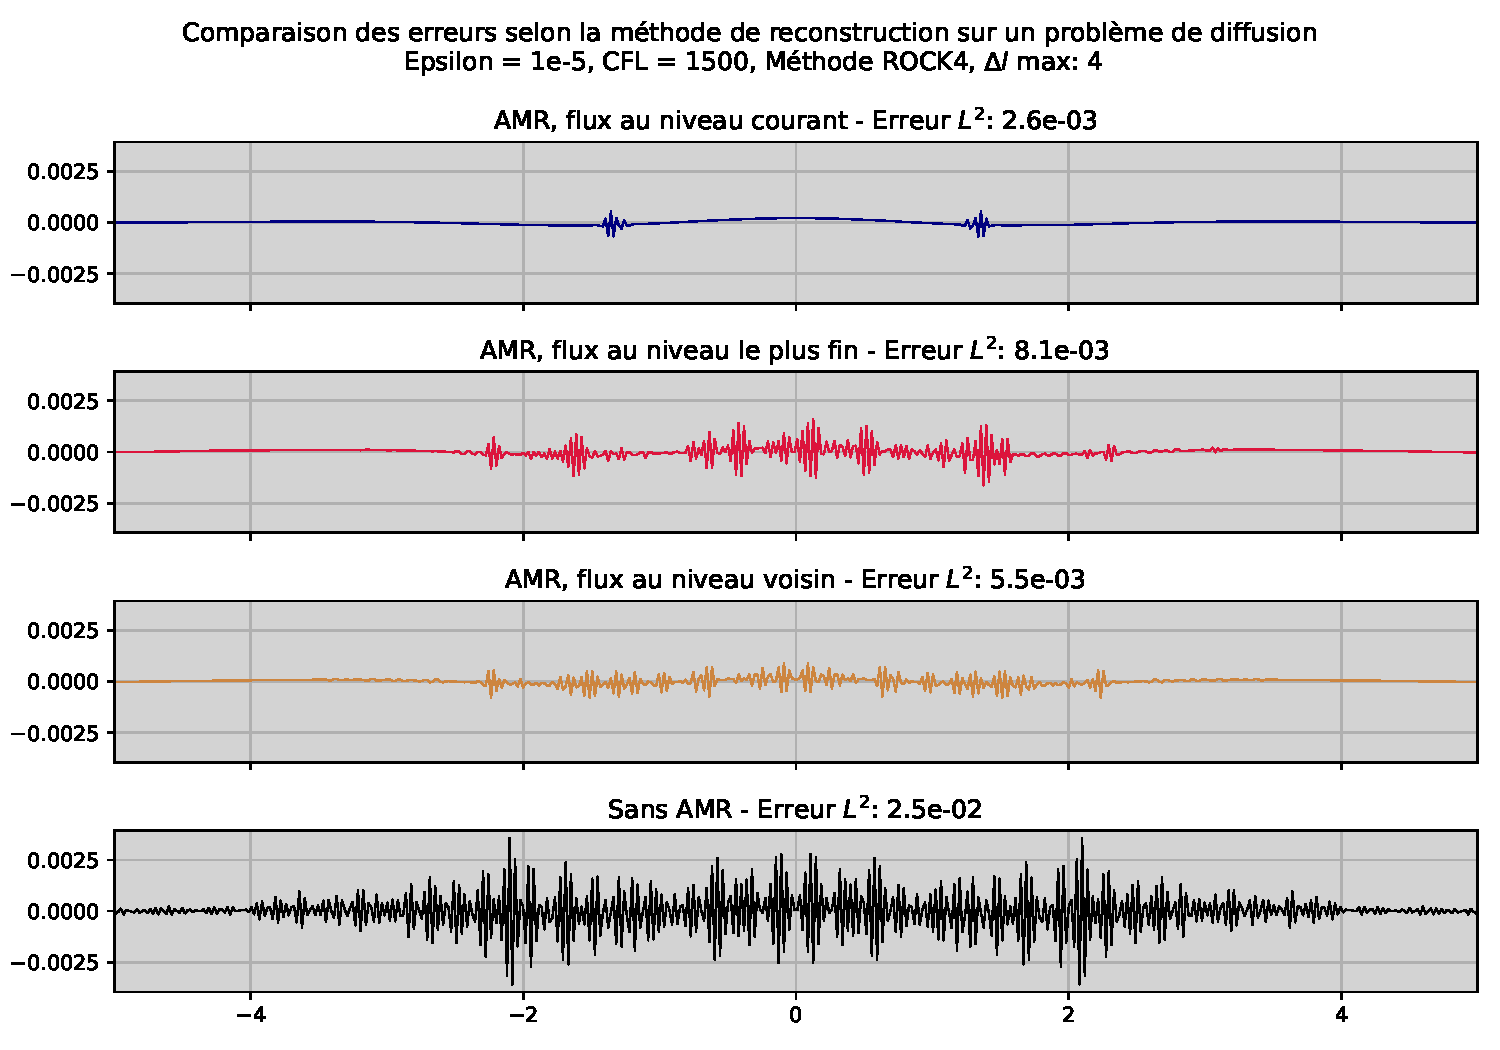
\includegraphics[width=\textwidth]{media/4_travail/3/Error_comparaison_according_to_flux_reconstruction_method.pdf}
    \caption{Erreur au pas de temps final pour les différentes méthodes, avec une constante CFL de diffusion $D\,\Delta t / \Delta x^2 = 1500$, correspondant à des solutions où l'erreur temporelle reste dominante.}
    \label{fig:erreur_diffusion_according_to_flux_recons_method}
    \end{figure}
    Si le paramètres de compression est très restrictif $\varepsilon = 10^{-5}$ (colonne de gauche), les 4 algorithmes sont équivalents, en effet il n'y a presque jamais d'adaptation de maillage, car le seuil de compression est trop restrictif.
    Pour des paramètres de compression plus raisonnables ($\varepsilon = 10^{-4}$ et $\varepsilon = 10^{-3}$), les observations sont plus riches.
    Lorsque les erreurs temporelles de dominent pas, les trois algorithmes d'AMR améliorent la convergence - ce qui est surprenant. Cependant leur convergence s'arrête plus tôt, du fait des 
    erreurs spatiales liées à l'AMR et pour des pas de temps assez petit, le schéma sans AMR demeure meilleur. Pour un pas de temps où l'erreur en temps domine, 
    en figure \ref{fig:flux_reconstruction_error} est tracé l'erreur au temps final pour chacune des méthodes est tracé et il semble effectivement que les méthodes avec AMR lissent
    "mieux" que la méthode sans AMR qui semble un peu plus bruité. 


    Pour des pas de temps menant à une erreur spatiale dominante, les résultats sont similaires à ce qui avait été observées, plus les flux sont évaluées à partir de reconstructions fines, 
    plus le plateau de saturation en erreur spatiales est important.
    \subsubsection{Conclusion}
    Deux conclusions sont à tirer de cette expérience:
    \begin{enumerate}
        \item L'AMR tend à faire chuter plus rapidement l'erreur temporelle qu'avec une méthode non adaptée spatialement, et cela indépendamment de la méthode d'évaluation du flux numérique.
        \item L'AMR mène à un plateau de convergence plus élevée que sans AMR (l'erreur spatiale domine). Ce qui est étonnant est que cette saturation de l'erreur arrive d'autant plus vite que les flux sont évaluées à partir de reconstructions fines; même observation qu'avec la méthode ERK2.
    \end{enumerate}
    Ces résultats ne valent a priori que sur une équation de diffusion "pure" et la relation d'ordre entre les erreurs qui parait incohérente n'est peut être que le résultat d'un 
    "heureux effet lissant" qu'apporte l'AMR et qui est plus prononcé encore si l'on évalue les flux au niveau courant (algorithme 1).
    La prochaine section se propose donc de reprendre l'expérimentation sur une équation de diffusion-réaction, présentant une onde progressive ce qui s'approche un peu plus
    d'un contexte de simulation industrielle réaliste.
    Dès lors, il ne s'agit plus pour le schéma de simplement lisser mais également suivre la dynamique d'un front d'onde ! Peut-être que les résultats seront différents.